\uuid{JspF}
\exo7id{7125}
\titre{exo7 7125}
\auteur{megy}
\organisation{exo7}
\datecreate{2017-02-08}
\isIndication{true}
\isCorrection{true}
\chapitre{Géométrie affine euclidienne}
\sousChapitre{Géométrie affine euclidienne du plan}

\contenu{
\texte{
% application directe
% angle inscrit et angle au centre, cas limite
% ou homothéties
Soient $\mathcal C$ et $\mathcal C'$ deux cercles tangents en un point $T$, et $\mathcal D_1$, $\mathcal D_2$ deux droites sécantes en $T$. On note $A$ et $A'$ (resp. $B$ et $B'$) les points d'intersection de $\mathcal D_1$ (resp. $\mathcal D_2$) avec $\mathcal C$ et $\mathcal C'$. Montrer que les droites $(AB)$ et $(A'B')$ sont parallèles.


\begin{center}
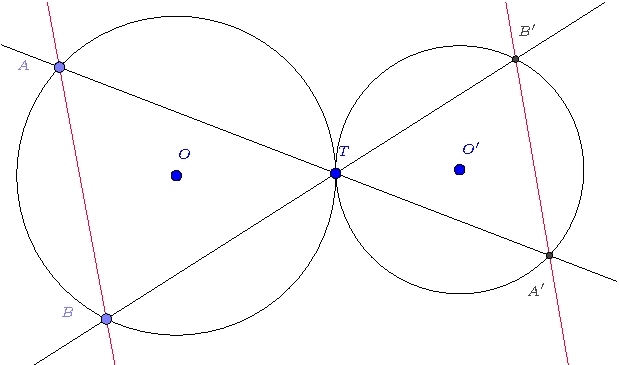
\includegraphics{../images/img007125-1}
\end{center}
}
\indication{Introduire la tangente commune $\mathcal T$ aux deux cercles. 
%Utiliser le cas limite du théorème de l'angle au centre.}
\reponse{
Soit $\mathcal T$ la tangente commune  aux deux cercles.

\begin{center}
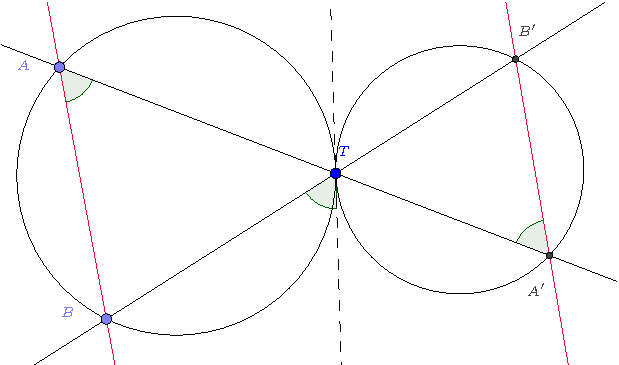
\includegraphics{../images/img007125-2}
\end{center}

Par le cas limite du théorème des angles inscrits, on a 
\[ (AB,AT) = (BT,\mathcal T)=(B'T,\mathcal T)=(A'B',A'T)\]

Comme $(AT) = (A'T)$, on en déduit que
\[ (AB,AT) = (A'B',AT),\]
et donc que $(AB)//(A'B')$. 

\underline{Autre preuve:} considérer une homothétie de centre $T$ qui envoie un cercle sur l'autre.
}
}
